
\section{Introduction}

\begin{figure}[!t]
    \centering
    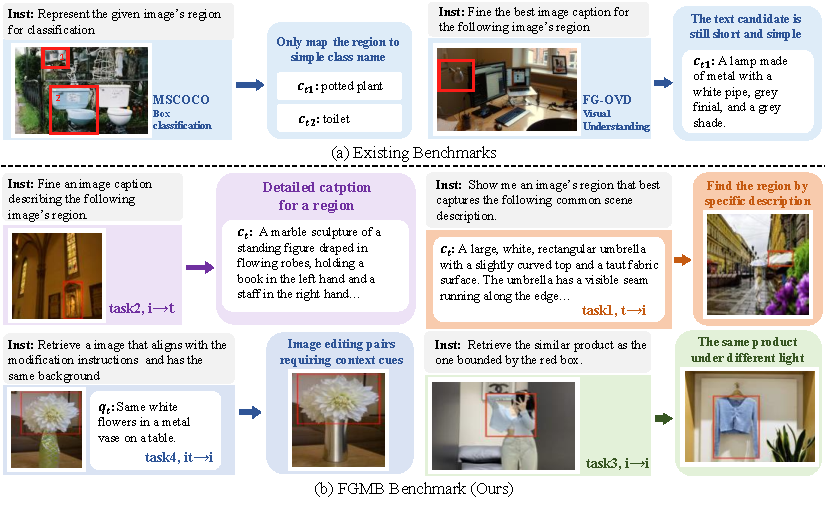
\includegraphics[width=\linewidth]{figures/fgmb-case.pdf}
    \caption{Examples of FGMB and existing benchmarks. Compared with FG-OVD and COCO, FGMB provides more complex query–candidate pairs and spans a wider range of modalities. }
    
    \label{fig:fgmb-case}
\end{figure}

In recent years, multimodal information retrieval has been widely applied in diverse real-world scenarios, such as E-commerce product search~\citep{jin2023eclip,dong2022m5product}, social media content recommendation~\citep{MVideoRec}, medical visual question answering~\citep{zhang2024biomedclip}, and content generation~\citep{yasunaga2022retrieval}. 
Existing studies largely fall into two categories. The first is the CLIP-based method, such as ~\citet{radford2021learning,zhai2023sigmoid,li2022blip}, which performs strongly on cross-modal tasks (e.g., image–text). The second is the VLM-based method~\citep{jiang2024vlm2vec,jiang2024e5v}, which extends the large language model's embedding capability to fused-modal retrieval (e.g., image–text-to-image).
However, the current research community mainly focuses on image-level retrieval, while ignoring region-level fine-grained retrieval, which is critical in real-world applications. For example, a shopper might upload a street photo and select the bounding box around a passerby's coat, prompting the system to retrieve similar products based on region-specific cues like shape, color, and brand.

Several existing methods make attempts to achieve fine-grained retrieval. Specifically， VLM-based methods~\citep{chen2025mmE5,liu2025lamra} are typically trained at the image level and are less effective in handling region-based prompts, which weakens their ability to capture fine-grained features. Although CLIP-based methods~\citep{xie2025fgclip,jing2024fineclip} enhance representations for dense prediction tasks through region-level contrastive learning with RoIAlign~\citep{matterport_maskrcnn_2017}, their fine-grained embeddings remain ineffective for large-scale retrieval. They also struggle to generate unified embeddings for fused-modal queries, requiring specialized modifications such as fusion layers in \citet{wei2023uniir}.

% In this work, we introduce LEMUR, a VLM-based framework for fine-grained multimodal retrieval. LEMUR incorporates the Region-aware Encoder (RAE), which consists of a ViT backbone and a projector. Independent of the VLM's native vision encoder. Moreover, through the layer-wise interactions\citep{he2018layer-wise} between the RAE and the , referred to as the context encoder (CE), LEMUR filters out background noise while retaining informative regional features. 
In this work, we introduce LEMUR, a VLM-based framework for fine-grained multimodal retrieval. Rather than relying solely on the VLM’s native vision encoder, LEMUR integrates a Region-Aware Encoder (RAE) that encodes image regions into highly detailed features. Importantly, the RAE and the native ViT employ separate projectors, preventing the regional features from interfering with the model’s native vision representations.
% The embeddings are projected into a separate space to avoid interference with native vision tokens, which would otherwise harm global-level representation. 
Furthermore, through layer-wise interactions~\citep{he2018layer-wise} between the RAE and the native encoder, LEMUR effectively captures detailed regional features while suppressing background noise.
To equip LEMUR with retrieval ability, we adopt a three-stage training strategy, including (1) RAE pretraining, which employs the Detailed Localized Captioning task~\citep{lian2025dam} under the next-token prediction paradigm to encourage the model to learn highly detailed regional representations; (2) Language-only contrastive learning, which converts the language generation capability of LLMs into embedding capability; and (3) Regional contrastive learning, which largely improves the fine-grained retrieval performance.

In addition, to facilitate training and provide a comprehensive evaluation framework, we establish a new benchmark named FGMB. This benchmark covers two meta-tasks and four multimodal retrieval scenarios~\citep{zhang2024gme}, targeting the challenge of retrieving the most relevant image or text given a query that specifies a region of interest. FGMB contains 225k region-level contrastive pairs, primarily derived from automatically annotated open-source web images~\citep{kakaobrain2022coyo-700m,kirillov2023segany}, image editing datasets ~\citep{vismin2024,jiao2024imgdiffcontrastivedatasynthesis}, and further enriched with a manually curated and privacy-sanitized subset from an image search database from a popular E-commerce platform\footnote{We are authorized by the company to obtain and share the data. The dataset is released under CC BYNC-SA 4.0 license and can be used for noncommercial purposes.}. All benchmark data will be released to support future research.

Extensive experiments validate the effectiveness of our approach and dataset. In the zero-shot setting, LEMUR directly combines the pretrained RAE with existing image-level VLM embedding models. Without any additional region-level contrastive training, LEMUR can surpass strong baselines in fine-grained retrieval tasks. Moreover, fine-tuning on the FGMB train set further enhances performance, yielding up to a 30\% improvement in region-level retrieval accuracy and providing gains for image-level retrieval tasks as well. In summary, our main contributions are as follows:

\begin{itemize}[leftmargin=*, itemsep=0em] 
\item We propose LEMUR, a VLM incorporating a Region-aware Encoder to process region-level prompts and produce fine-grained visual tokens. We further design a three-stage training pipeline to strengthen LEMUR's fine-grained understanding and embedding ability. LEMUR achieves state-of-the-art performance in the zero-shot setting, and its effectiveness can be further boosted through region-level contrastive training, while also slightly improving image-level retrieval.


\item We construct FGMB, a fine-grained multimodal retrieval benchmark comprising 225k high-quality contrastive pairs, organized into two meta-tasks and four representative retrieval scenarios. %The dataset integrates auto-annotated web images with a manually curated and privacy-sanitized subset from ???, addressing the limitations of existing benchmarks such as limited task diversity, overly coarse granularity, and the absence of descriptive regional annotations. Importantly, % 
It provides data for both training and evaluation, enabling comprehensive evaluation and facilitating deployment of fine-grained multimodal retrieval methods.
\end{itemize}